\section{Services}
\subsection{Zeitmessung}

\begin{figure}[ht]
  \centering
  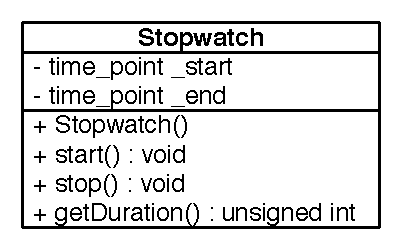
\includegraphics{04_Implementierung/00_media/Stopwatch.pdf}
  \caption{Klassendiagramm: Stopwatch}
  \label{ClassStopwatch}
\end{figure}

Wie bereits in Abb. \ref{Ablauf} dargestellt, wird die Zeitmessung, die durch die Klasse Stopwatch (vgl. Abb. \ref{ClassStopwatch}) durchgeführt wird, nach der Konfiguration zuerst instantiiert und dann mit der Methode \texttt{start()} gestartet. Sobald alle Pläne expandiert und die Kosten berechnet sind, wird die Messung durch die Methode \texttt{stop()} beendet. Um eine möglichst genaue Messung durchführen zu können, wurde die Uhr \texttt{std::chrono::steady\_clock} verwendet. Diese Uhr ist Teil von C++11. Wie in der Dokumentation \cite{cppreference_2015_clock} beschrieben, handelt es sich bei der Uhr um eine monotone Uhr. Sie kann nicht rückwärts laufen, solange die physische Zeit fortfährt. Die Uhr selbst mit der Wall\-Clock\-Time verbunden, ist das passende Werkzeug zur Messung von Intervallen. 

Die Dauer zwischen Start der Expansion und dem Ende der Kostenberechnung wird in Nanosekunden gemessen und mit der Methode \texttt{getDuration()} ausgegeben, um ein möglichst akkurates Ergebnis zu erhalten. Die gemessenen Ergebnisse werden sowohl als Debug-Log in der Konsole ausgegeben, als auch  in einem Log File gespeichert.




\subsection{Logging und Debugging}
Zum Debugging wurde auch eine externe Bibliothek eingesetzt: EasyLogging++ \cite{easylogging}, ein einfach zu bedienendes, jedoch hochgradig konfigurierbares Logging Instrument. Gerade die Leichtgewichtigkeit - das Tool besteht nur aus einer Headerklasse -, die einfache Bedienung und die Geschwindigkeit gaben  den Ausschlag zur Nutzung der Library. Mit Hilfe dieser Library werden debugging Informationen geschrieben, aber auch Zeitmessungen gespeichert, Pläne ausgegeben und sonstige Debugging Nachrichten ausgegeben. Insbesondere ist die Unterscheidung zwischen unterschiedlichen Debug\-Leveln wichtig. Auf mehreren Ebenen (INFO, WARNING, DEBUG, etc.) können Informationen ausgegeben werden. Je nachdem welches Level angesprochen ist, werden nur Informationen über dieses ausgegeben. 

\subsection{Operatoren und Operations}
Wie in Abb. \ref{PlanNodeClass} zu sehen, sind zwei Operatoren vorgesehen JOIN und SCAN. Um aus ihnen im Zusammenhang mit Planknoten und Äquivalenzklassen Pläne herzustellen, wurde die Klasse \texttt{Operations} (vgl. \ref{ClassOperations} erstellt. Diese Klasse bietet einfachen Zugriff auf die meist verwendeten Arten von Äquivalenzklassen und Planknoten. Wird beispielsweise mit der Methode \texttt{scan} direkt eine Äquivalenzklasse mit einer bestimmten Relation, ein übergeordneter Planknoten und eine wiederum übergeordnete Äquivalenzklasse erstellt werden.

Neben diesen Operator steht auch ein Oprator zur Erzeugung von Joins mit und ohne übergeordneter Äquivalenzklasse zur Verfügung \texttt{join} resp. \texttt{joinPN}.

Um Kosten bei der Erzeugung neuer Objekte zu sparen, werden alle Planknoten und Äquivalenzklassen in Resourvars angelegt. Es werden also bereits vor Start des eigentlichen Tests alle Instanzen gebildet und während der Laufzeit mit konkreten Daten gefüllt.

